\documentclass[a4paper]{article}

%% Language and font encodings
\usepackage[english]{babel}
\usepackage[utf8x]{inputenc}
\usepackage[T1]{fontenc}

%% Sets page size and margins
\usepackage[a4paper,top=3cm,bottom=2cm,left=3cm,right=3cm,marginparwidth=1.75cm]{geometry}

%% Useful packages
\usepackage{amsmath}
\usepackage{graphicx}
\usepackage{caption}
\usepackage{subcaption}
\usepackage[colorinlistoftodos]{todonotes}
\usepackage[colorlinks=true, allcolors=blue]{hyperref}

\title{Evaluación 2: El Atractor de Lorenz, ejemplo de Caos dinámico. }
\author{Jesús Antonio González Espinosa \\ \\ Física Computacional 1}
\date{26 de Abril del 2018}

\begin{document}
\maketitle

\section{Introducción}
El sistema de ecuaciones diferenciales ordinarias de Lorenz son una serie de ecuaciones, estudiadas por Edward Lorenz, que definen un modelo matemático que simplifican la convención atmosférica. Las ecuaciones de Lorenz son tres:

\begin{center}
$\frac{dx}{dt} = \sigma(y-x)$,

$\frac{dy}{dt} = x(\rho - z) - y$,

$\frac{dz}{dt} = xy - \beta z$.
\end{center}

Éstas ecuaciones, en particular, describen el ratio de cambio de tres cantidades con respecto al tiempo. Además de servir para la convección atmosféricas, también tiene más usos en los modelos de laseres, dinamos, termosifones, y otras áreas de la física.

Como en las actividades anteriores, esté sistema de ecuaciones tiene soluciones son caóticas; y es lo que se va a ejemplificar en esta segunda evaluación, a partir de un código de Python de Goeff Boeing.

\pagebreak


\section{Resultados}
La evaluación consiste de cuatro pasos a seguir, donde se presentan tres diferentes combinaciones de valores para sigma, beta y rho; para posteriormente presentar una animación y gráficas bi-dimensionales para X, Y y Z de sus fases, y sus posiciones con respecto al tiempo. 

\subsection{Primer Caso}
Para el primer caso, se ha utilizado los valores de:
$\sigma$ (Sigma) = 10, $\beta$ (Beta) = 8/3 y $\rho$ (Ro) = 28. 

\begin{figure}[h!]
  \centering
  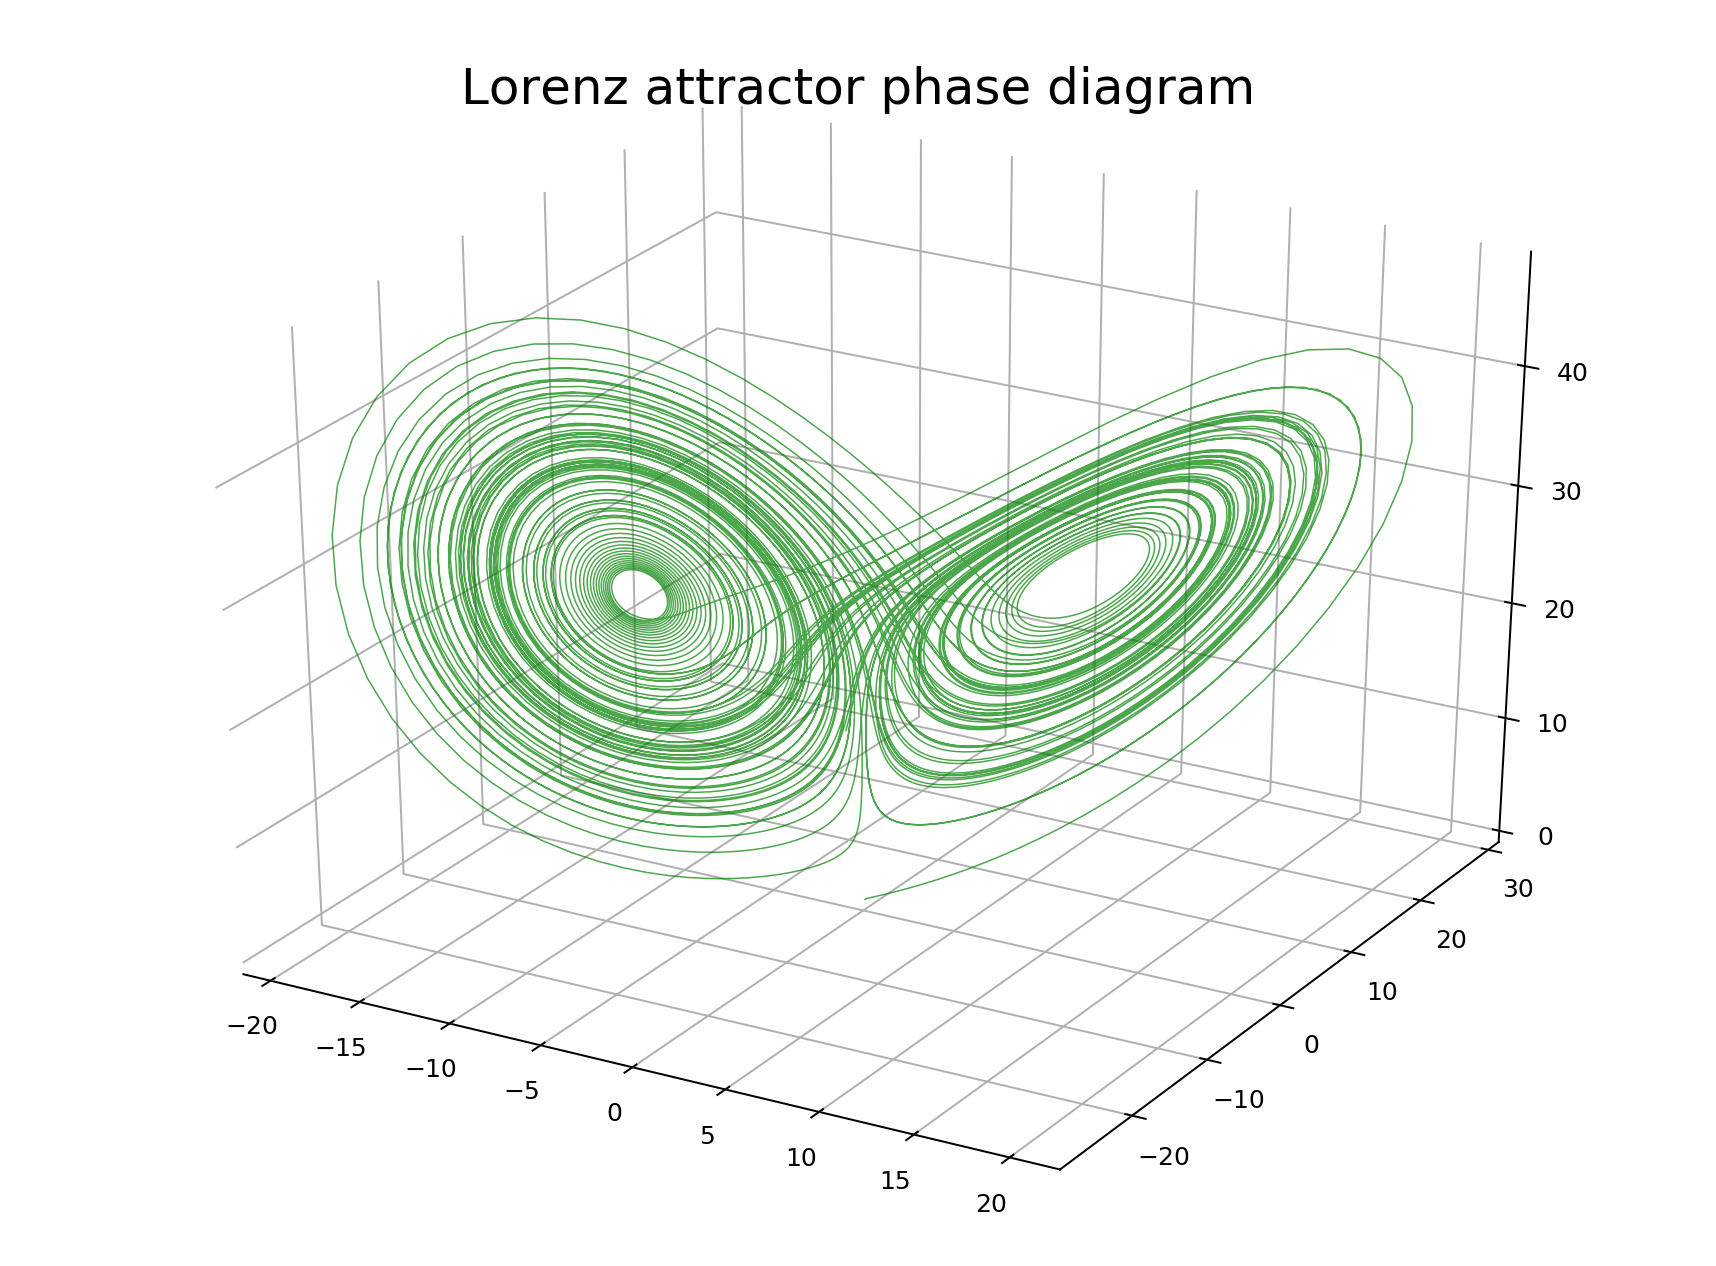
\includegraphics[width=0.8\linewidth]{lorenz-attractor-3d1.png}
   \caption{Gráfica de Fase del Atractor de Lorenz}
\end{figure}

La primera imagen generada por el código ilustra la gráfica de X, Y y Z, que nos presenta la Fase del atractor de Lorenz en tres dimensiones. 

Ahora, el código genera las fases presentadas en los planos:
\begin{figure}[h!]
  \centering
  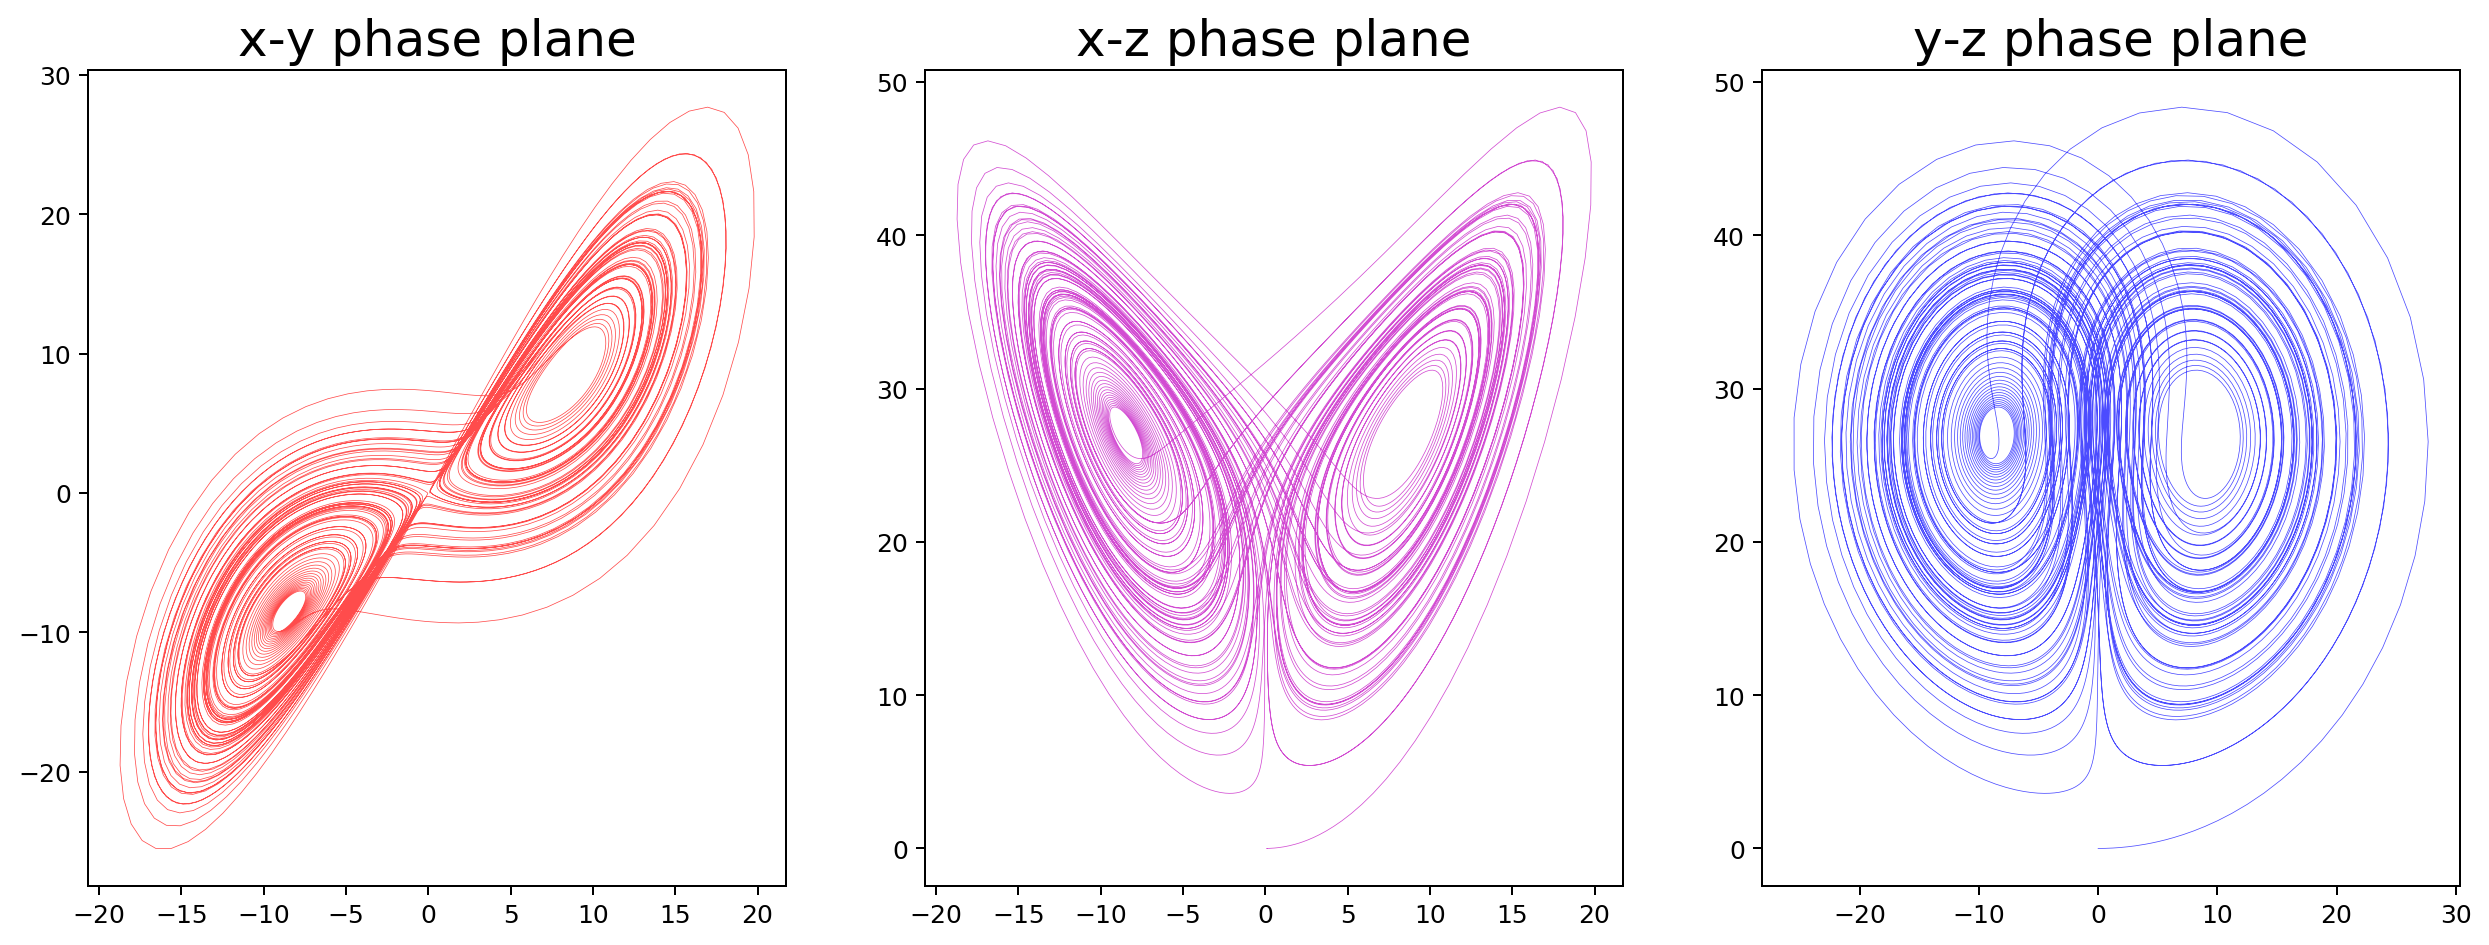
\includegraphics[width=0.6\linewidth]{lorenz-attractor-phase-plane1.png}
   \caption{Gráfica de Fase del Atractor de Lorenz en los planos.}
\end{figure}

La imagen nos presentan las fases en los planos XY, XZ y YZ respectivamente, lo que nos complementa perfectamente la gráfica en el espacio, ya que nos da mayor perspectiva de tal. Podemos ver como las soluciones caóticas nos generan una forma de alas de mariposa. 

\pagebreak

Por último tenemos:

\begin{figure}[ht!]
  \centering
  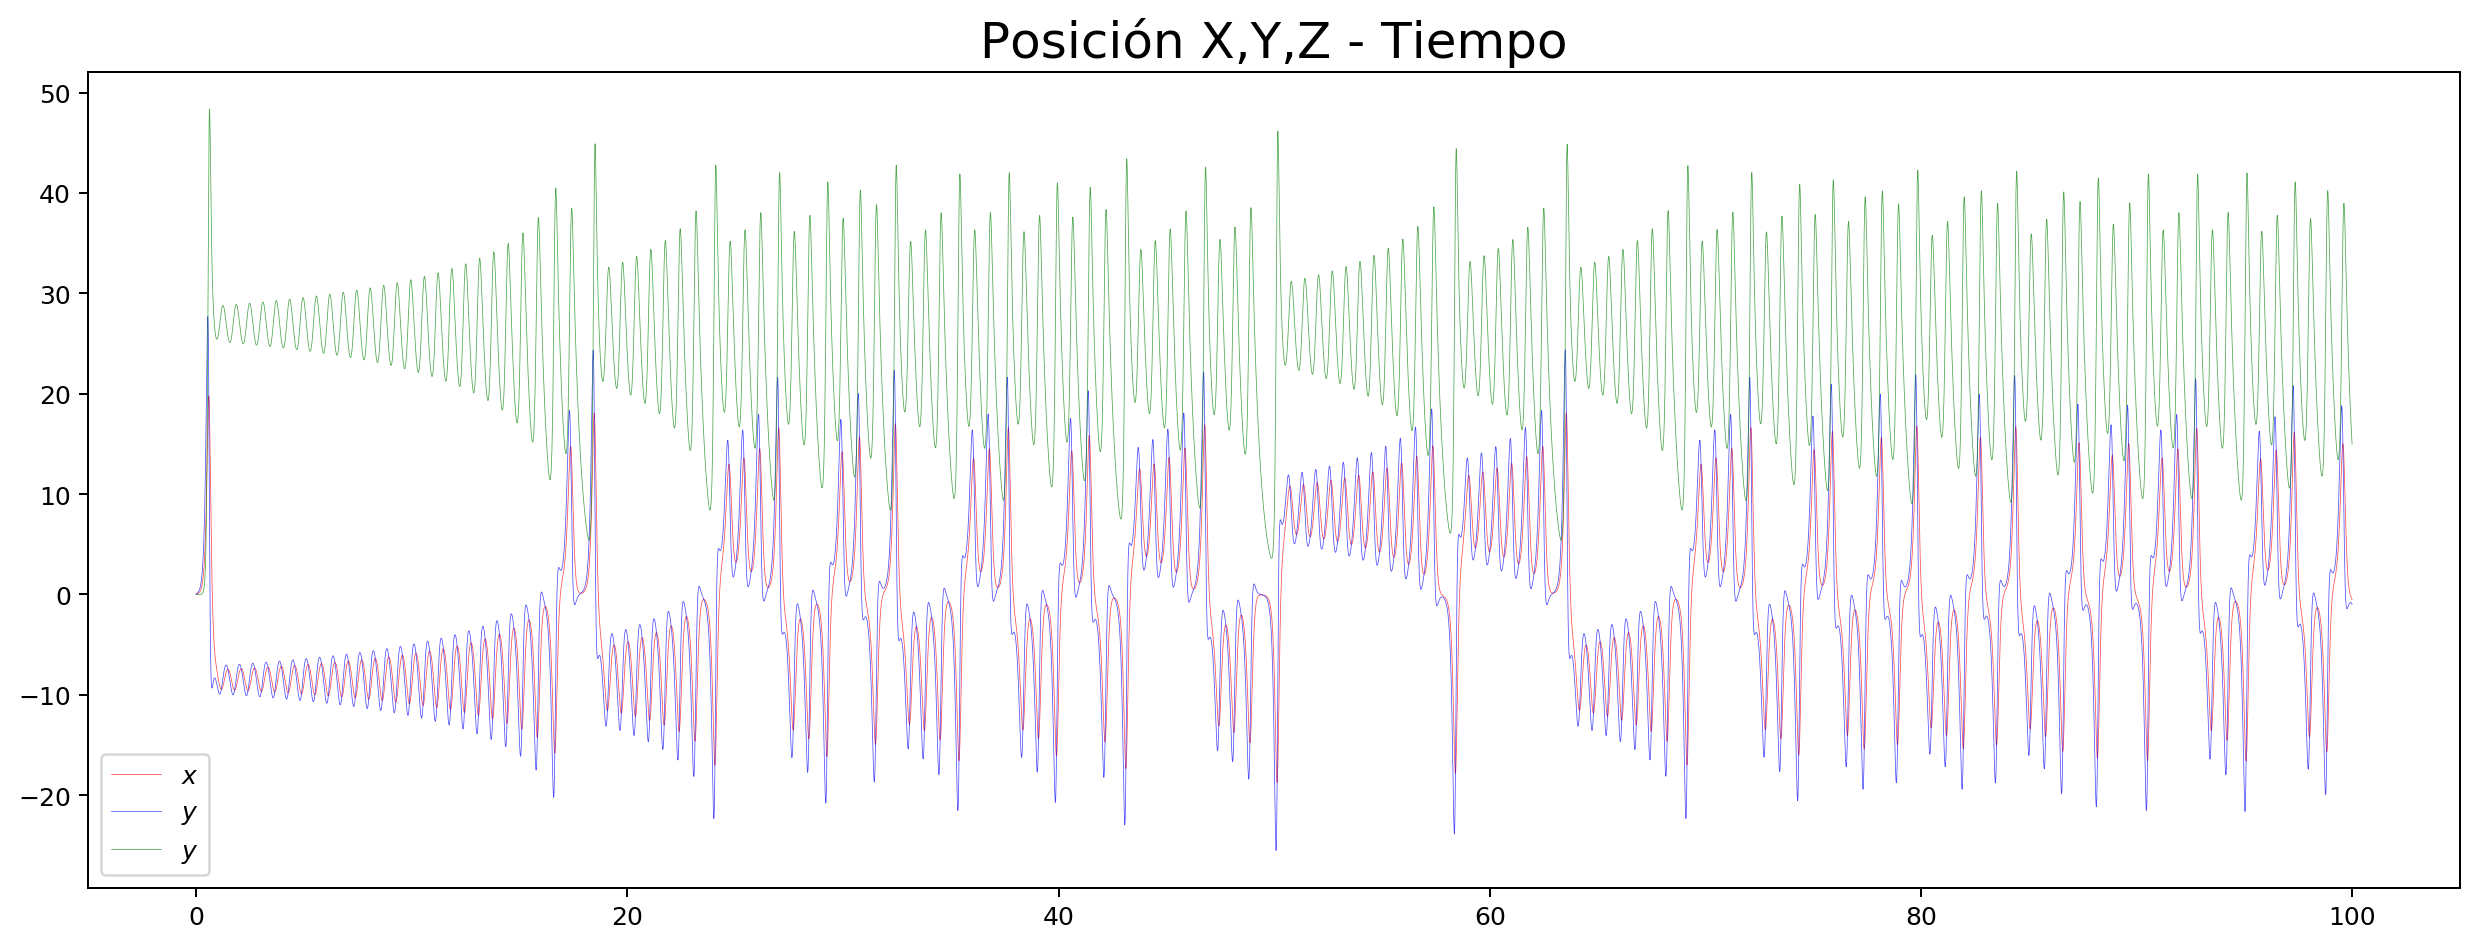
\includegraphics[width=0.6\linewidth]{lorenz-posicion-tiempo1.png}
   \caption{Posición con respecto al Tiempo}
\end{figure}

\begin{figure}[ht!]
  \centering
  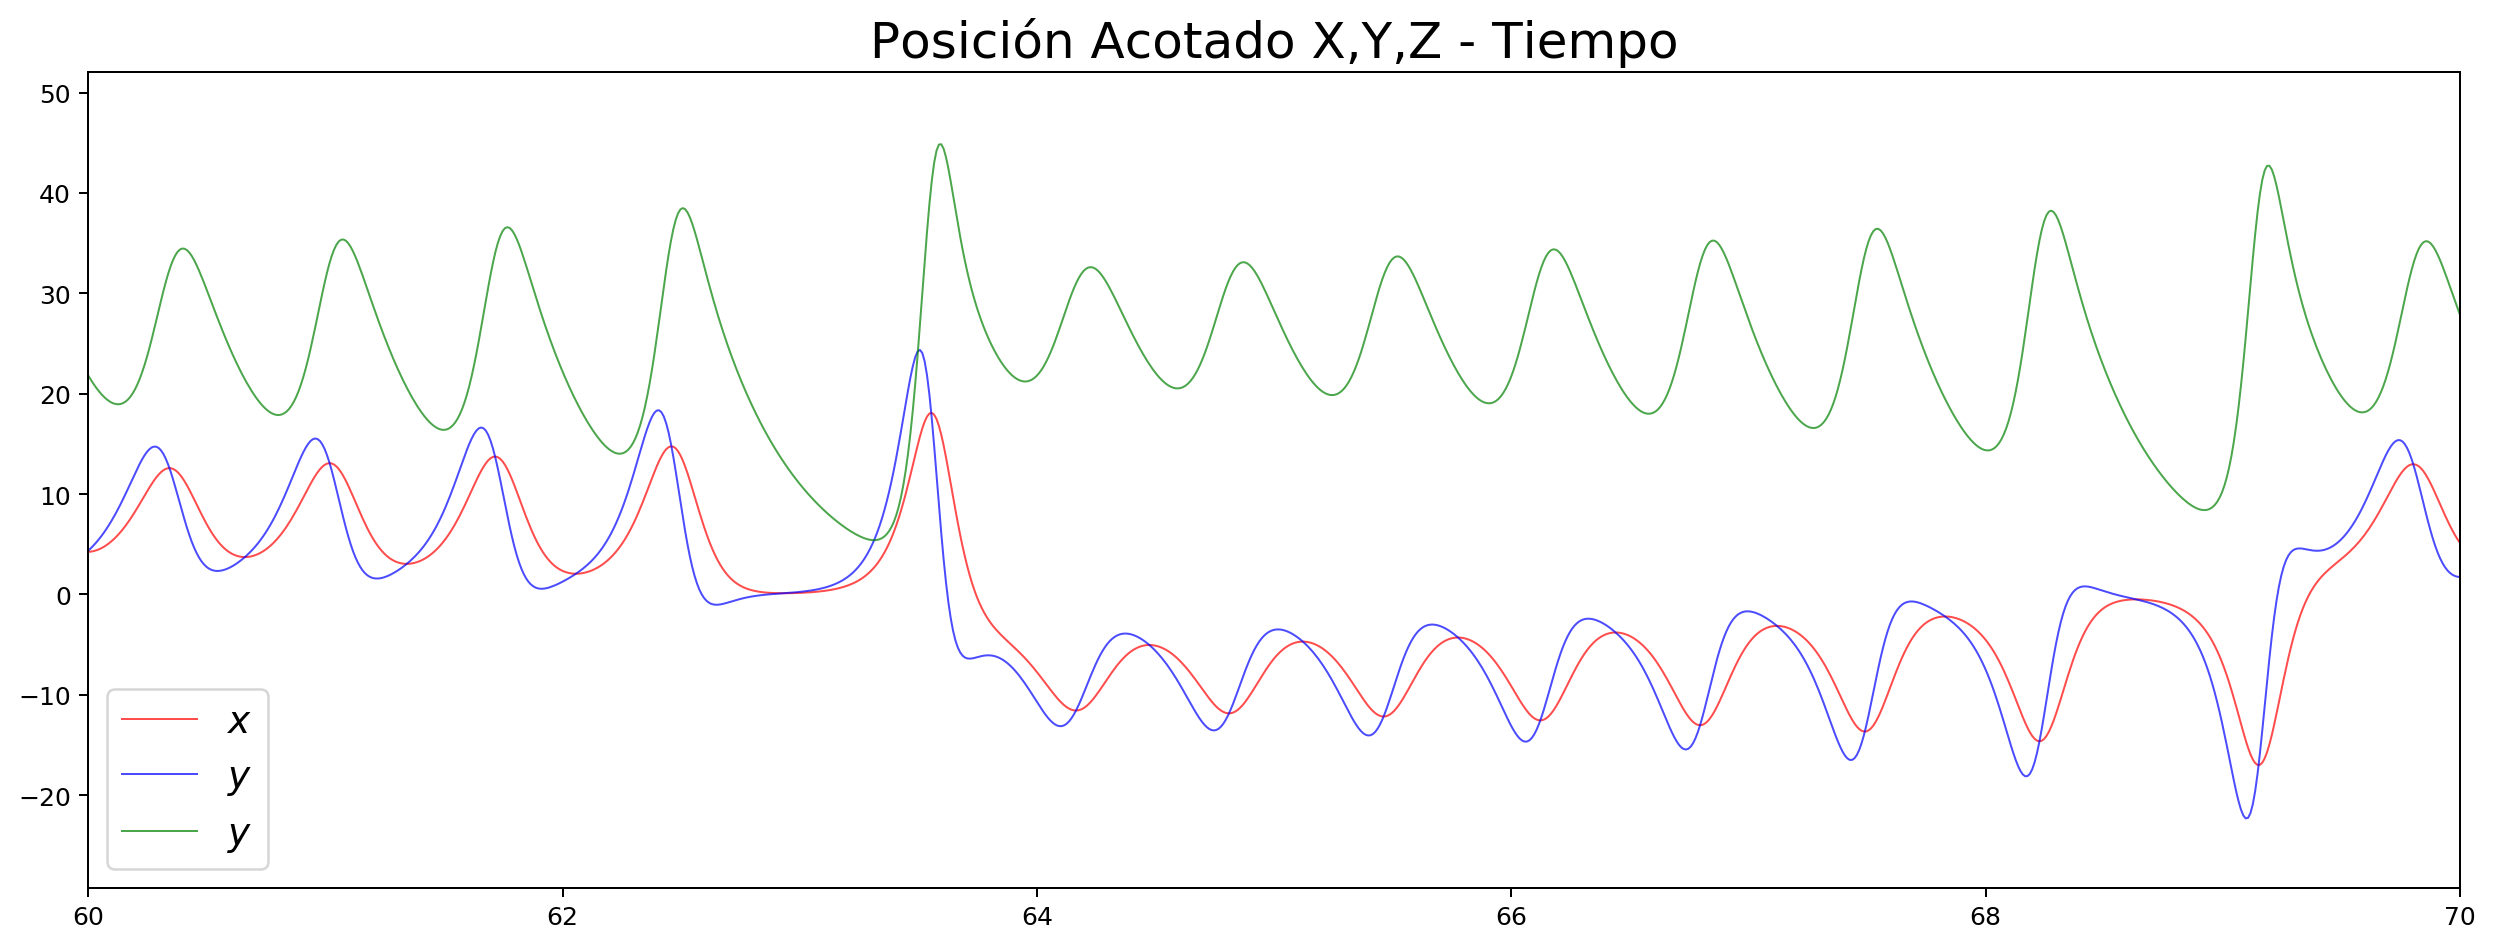
\includegraphics[width=0.6\linewidth]{lorenz-posicion-acotado-tiempo1.png}
  \caption{Posición con respecto al Tiempo}
\end{figure}

Aquí podemos observar las gráficas de posición de X, Y y Z con respecto al tiempo. En la segunda gráfica se acota el tiempo, para pode apreciar como X y Y se comportan muy parecido, mientras que Z está en valores más altos. 

\subsection{Segundo Caso}
Para el segundo caso, se ha utilizado los valores de:
$\sigma$ (Sigma) = 28, $\beta$ (Beta) = 4 y $\rho$ (Ro) = 46.92. 

\begin{figure}[h!]
  \centering
  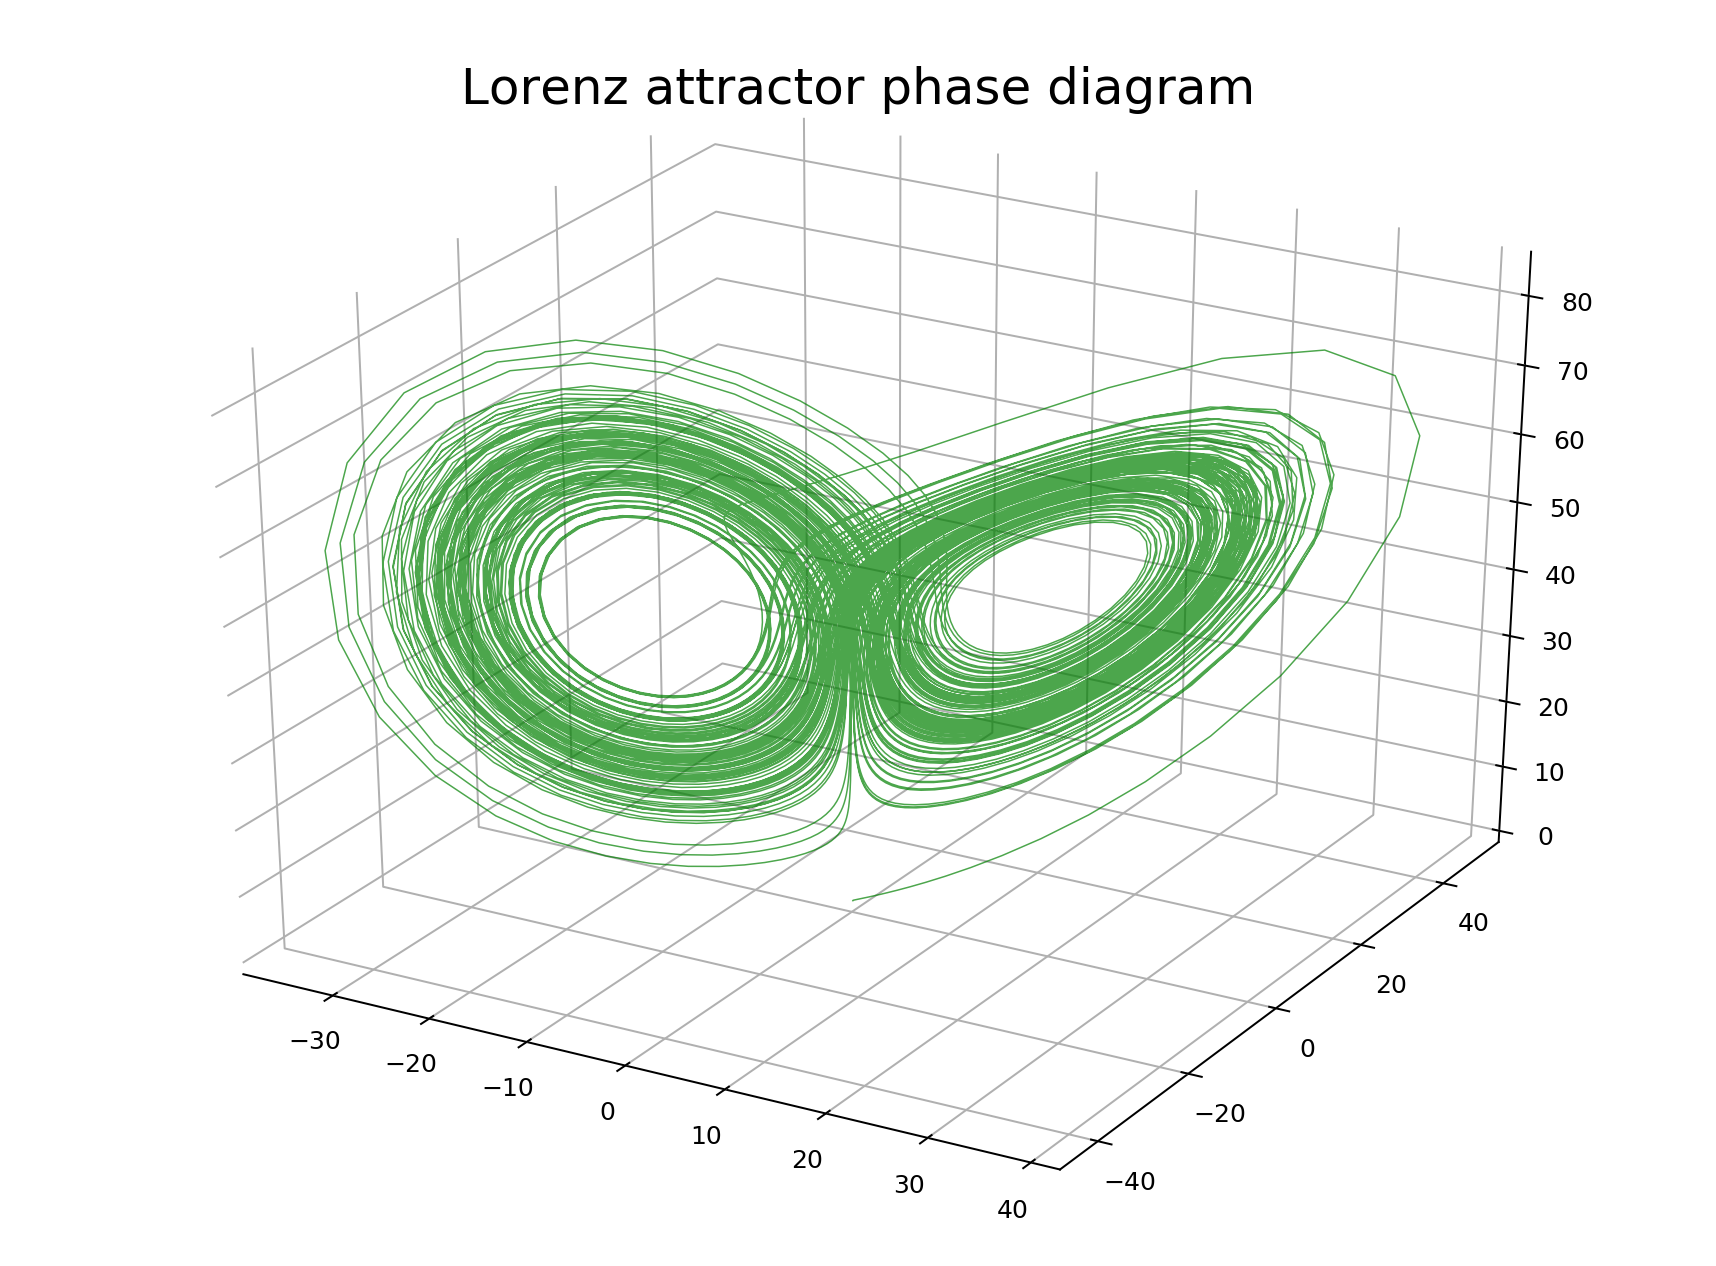
\includegraphics[width=0.8\linewidth]{lorenz-attractor-3d2.png}
   \caption{Gráfica de Fase del Atractor de Lorenz}
\end{figure}

Esta gráfica de Fase del Atractor es muy parecida a la del primer caso, solo que ahora tiene una forma más parecida a un ocho o un infinito, porque está mas concentrado en un camino, dejando huecos que le dan esta forma mencionada.

Ahora, el código genera las fases presentadas en los planos:
\begin{figure}[h!]
  \centering
  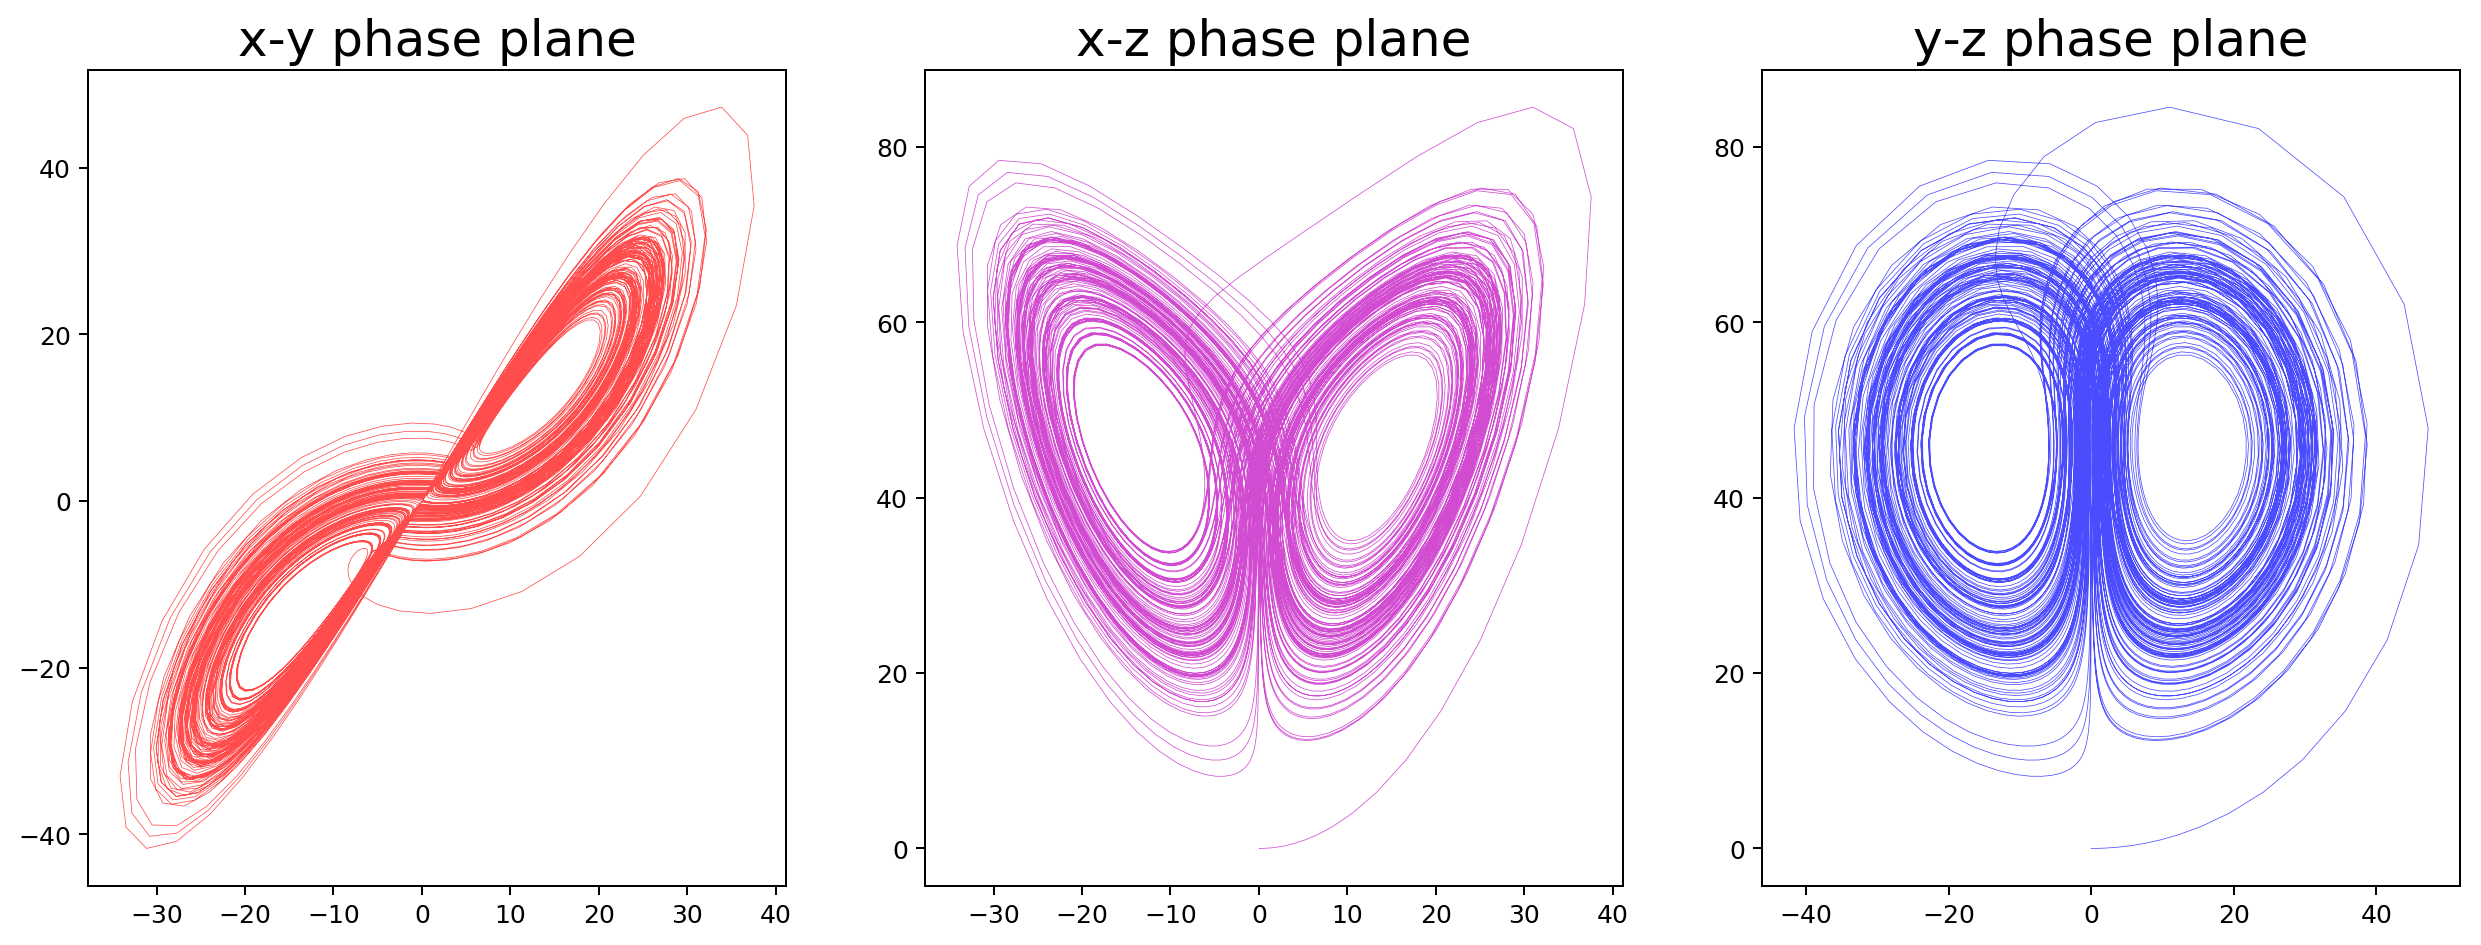
\includegraphics[width=0.6\linewidth]{lorenz-attractor-phase-plane2.png}
   \caption{Gráfica de Fase del Atractor de Lorenz en los planos.}
\end{figure}

La imagen nos presentan las fases en los planos XY, XZ y YZ respectivamente, que también se parecen mucho a los planos de la fase del primer caso, solo que más concentrados. También podemos observar que en el plano XZ, aun parece haber una forma de mariposa, a pesar de no dar esa perspectiva en la gráfica en el espacio. 

Por último tenemos:

\begin{figure}[ht!]
  \centering
  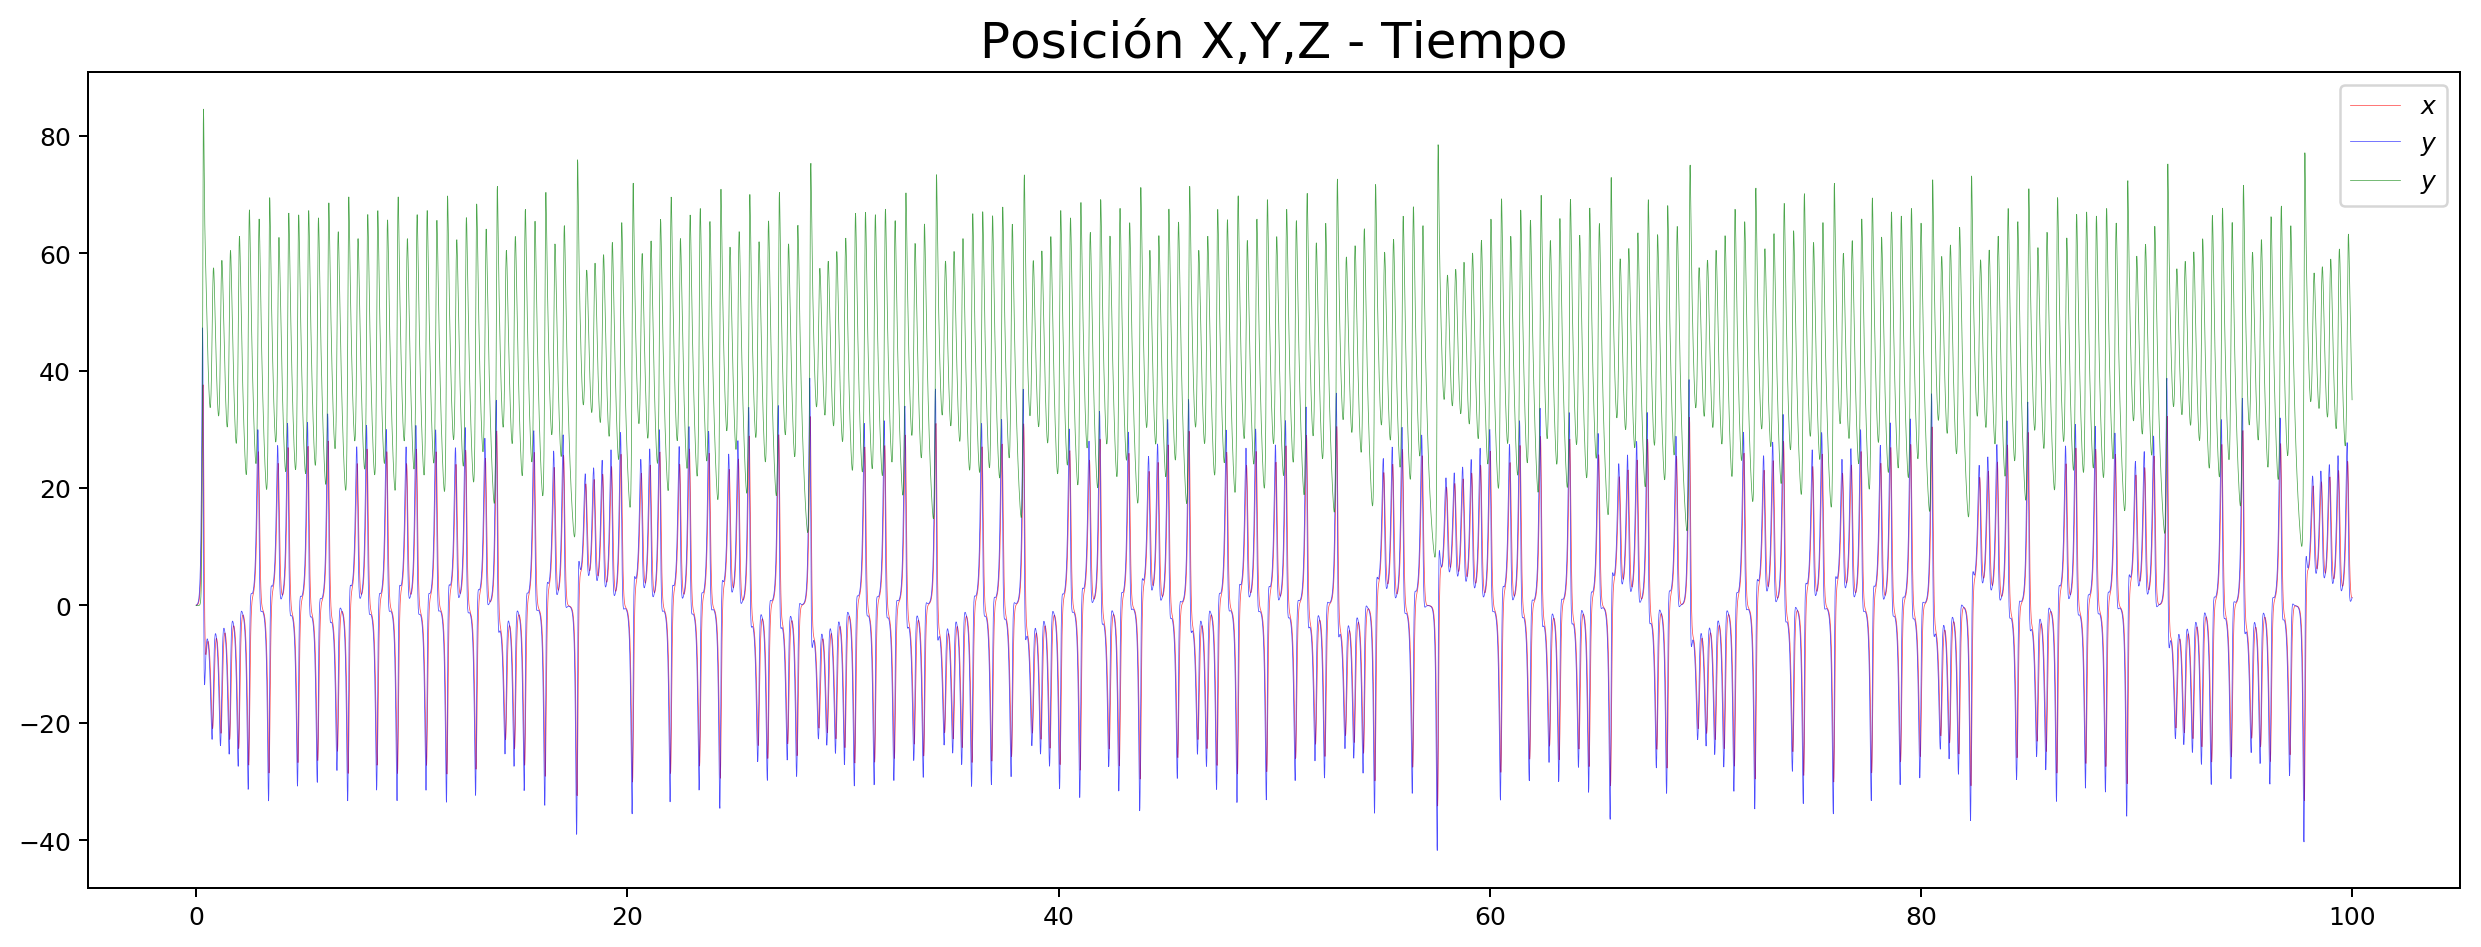
\includegraphics[width=0.6\linewidth]{lorenz-posicion-tiempo2.png}
   \caption{Posición con respecto al Tiempo}
\end{figure}

\begin{figure}[ht!]
  \centering
  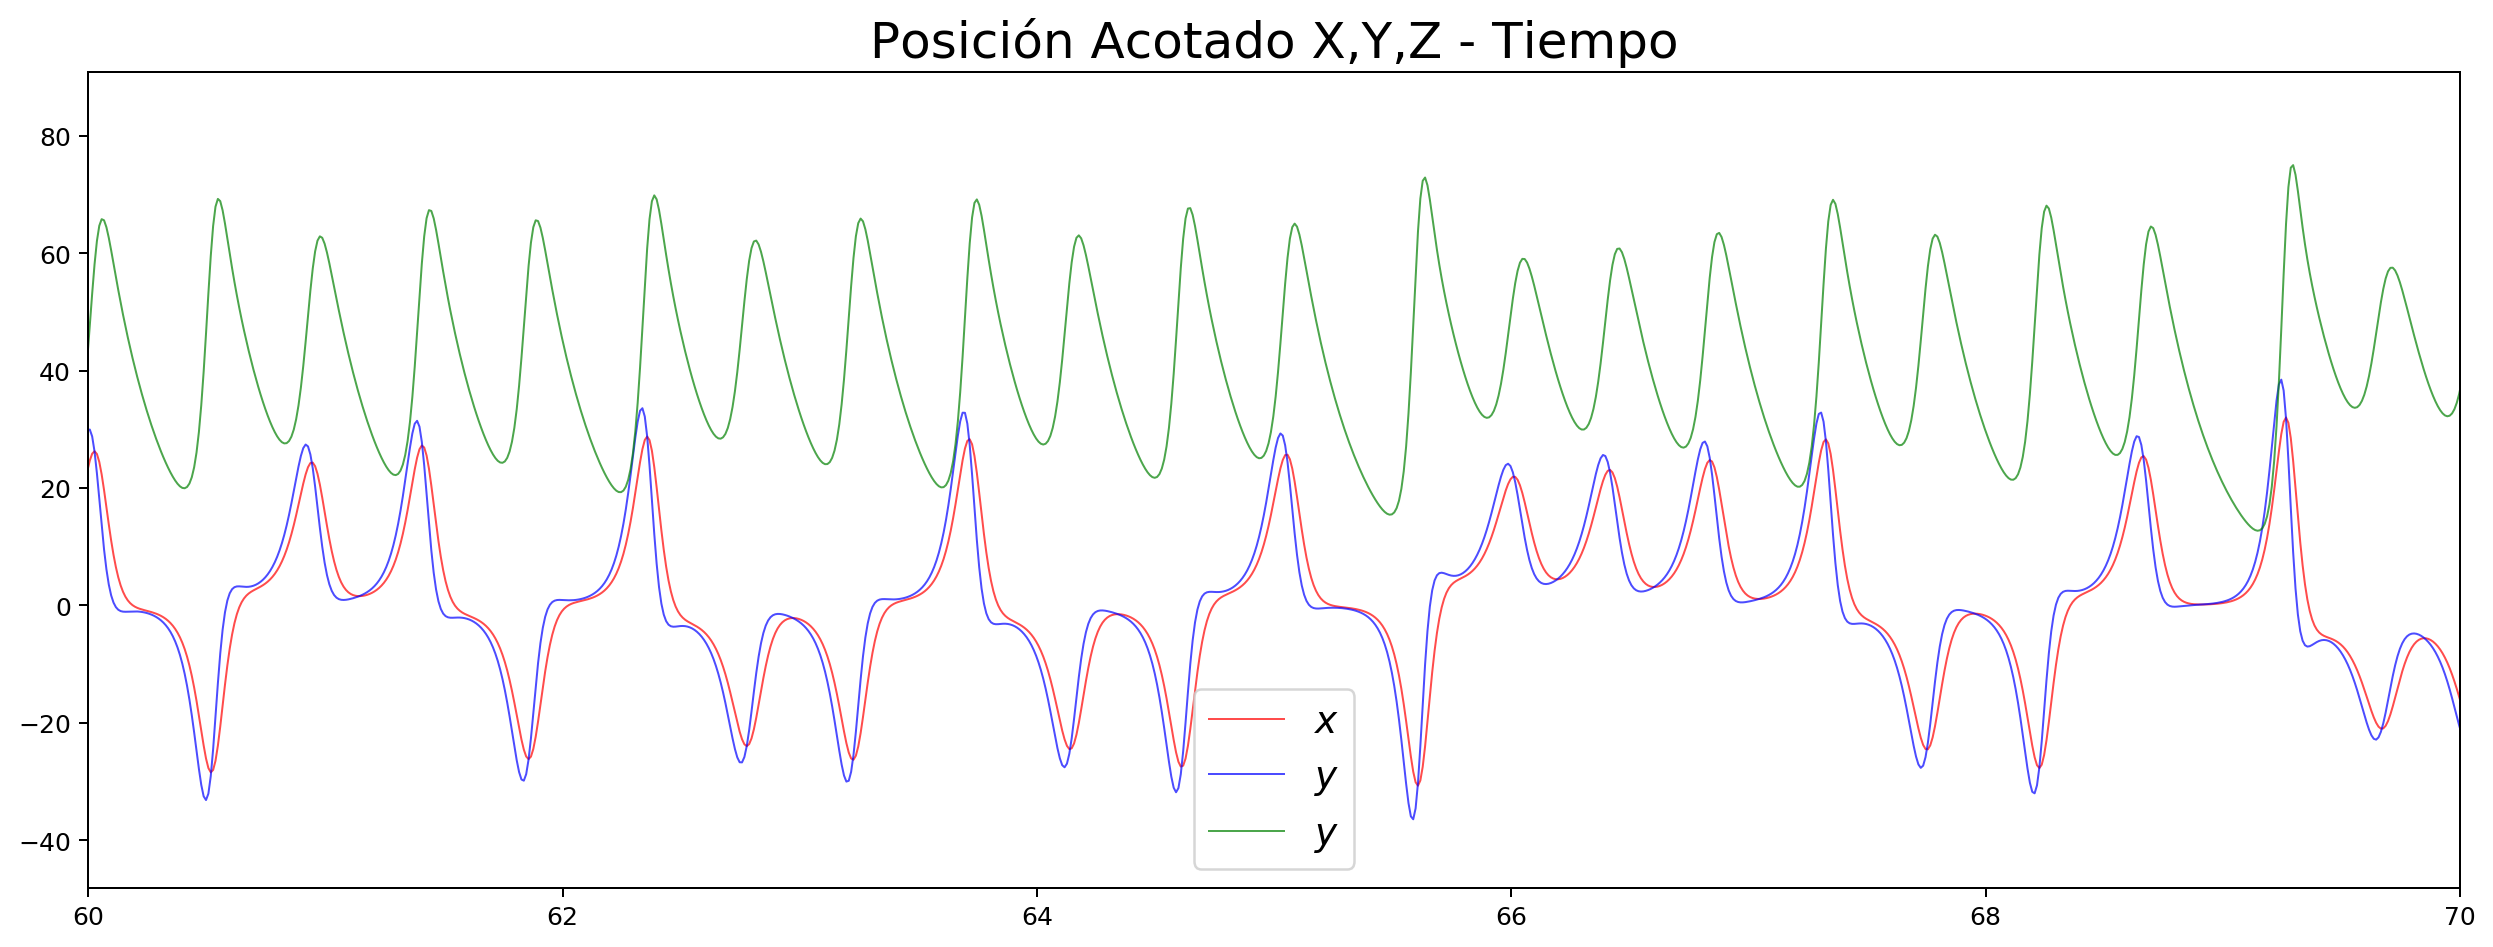
\includegraphics[width=0.6\linewidth]{lorenz-posicion-acotado-tiempo2.png}
  \caption{Posición con respecto al Tiempo}
\end{figure}

Aquí podemos observar las gráficas de posición de X, Y y Z con respecto al tiempo. En la segunda gráfica, donde mostramos más de cerca las posiciones, podemos notar que X y Y siguen teniendo un camino muy unido, pero de forma diferente al del primer caso, mientras que Z sigue estando más elevado.

\pagebreak

\subsection{Tercer Caso}
Para el tercer caso, se ha utilizado los valores de:
$\sigma$ (Sigma) = 10, $\beta$ (Beta) = 8/3 y $\rho$ (Ro) = 99.96. 

\begin{figure}[h!]
  \centering
  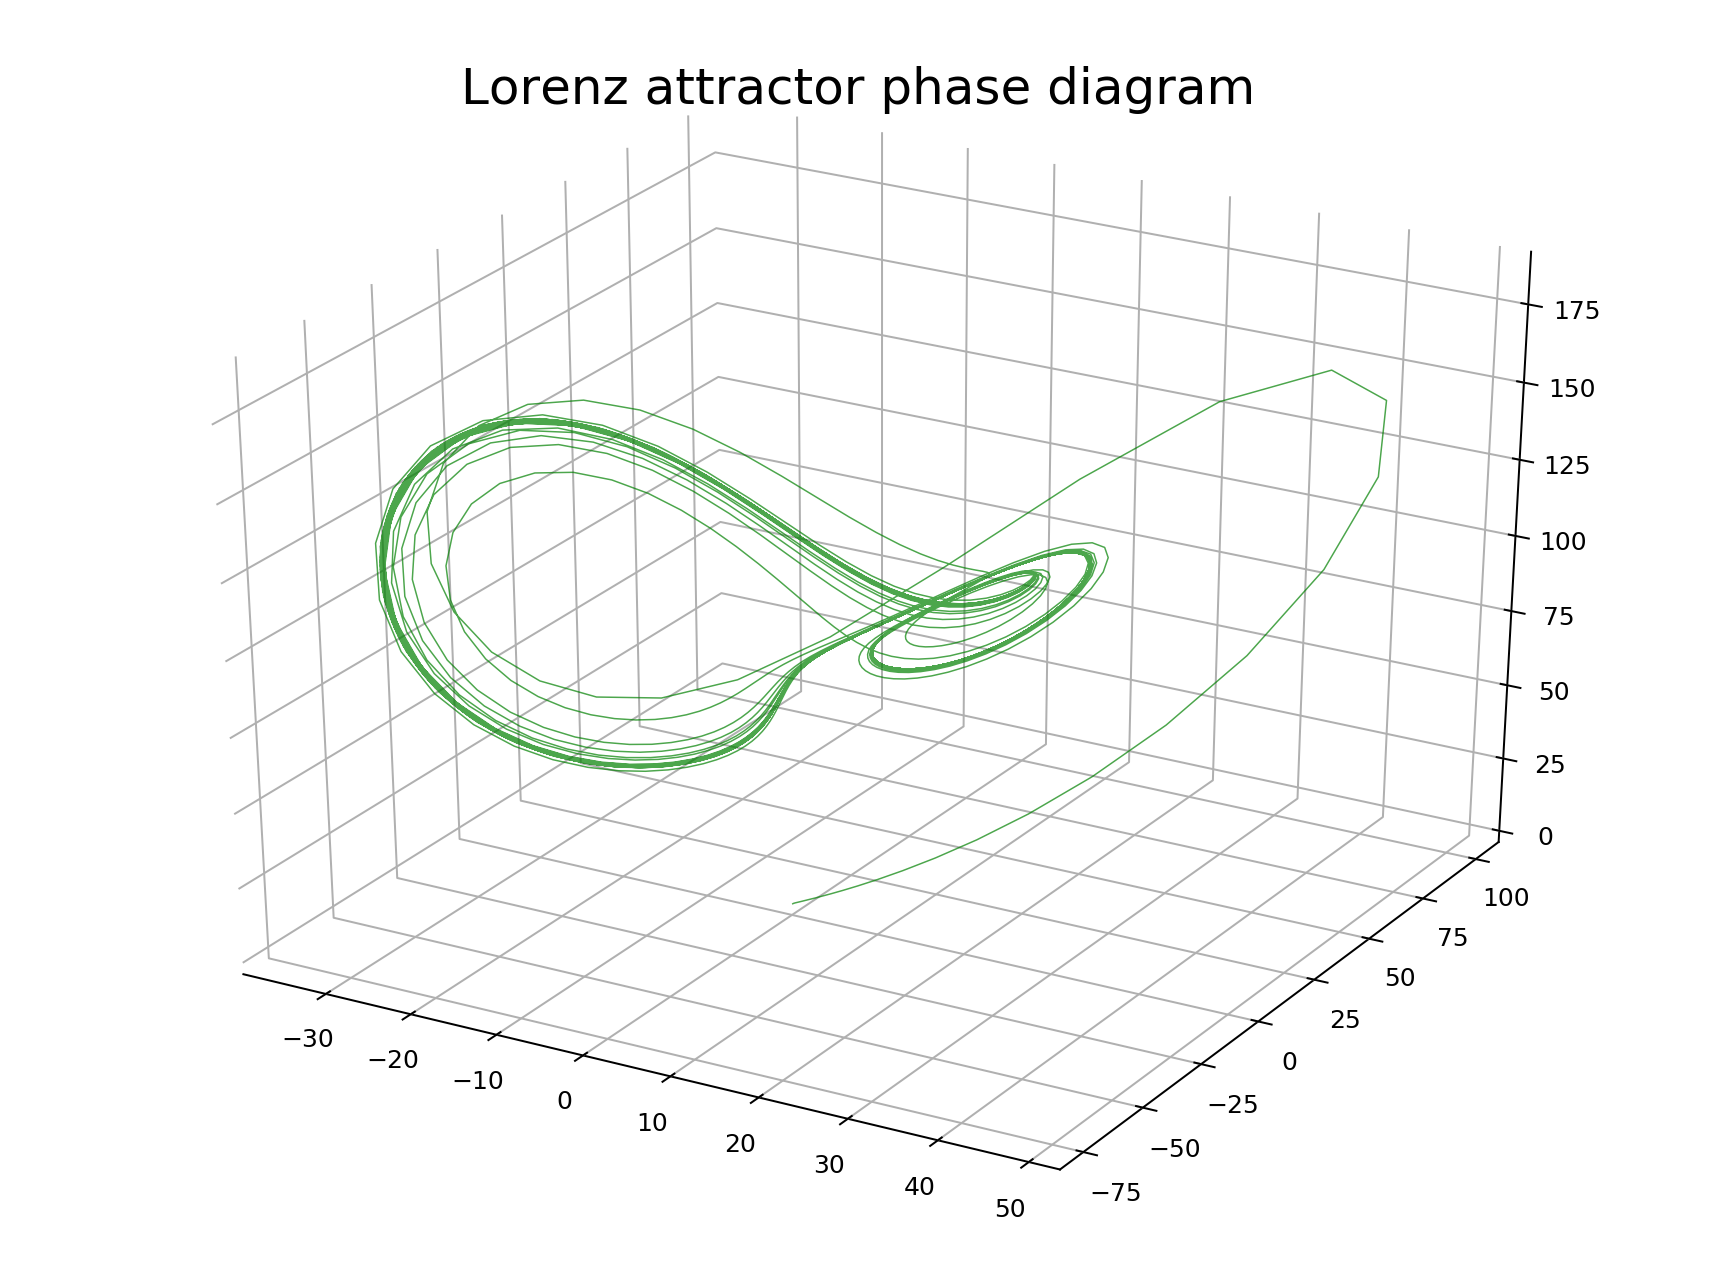
\includegraphics[width=0.8\linewidth]{lorenz-attractor-3d3.png}
   \caption{Gráfica de Fase del Atractor de Lorenz}
\end{figure}

Esta gráfica de Fase del Atractor es diferente a las primeras dos, ya que muestra estar más concentrada hacia un lado, dejando de mostrar formas tan definidas de alas de mariposa u ochos.  

Ahora, el código genera las fases presentadas en los planos:
\begin{figure}[h!]
  \centering
  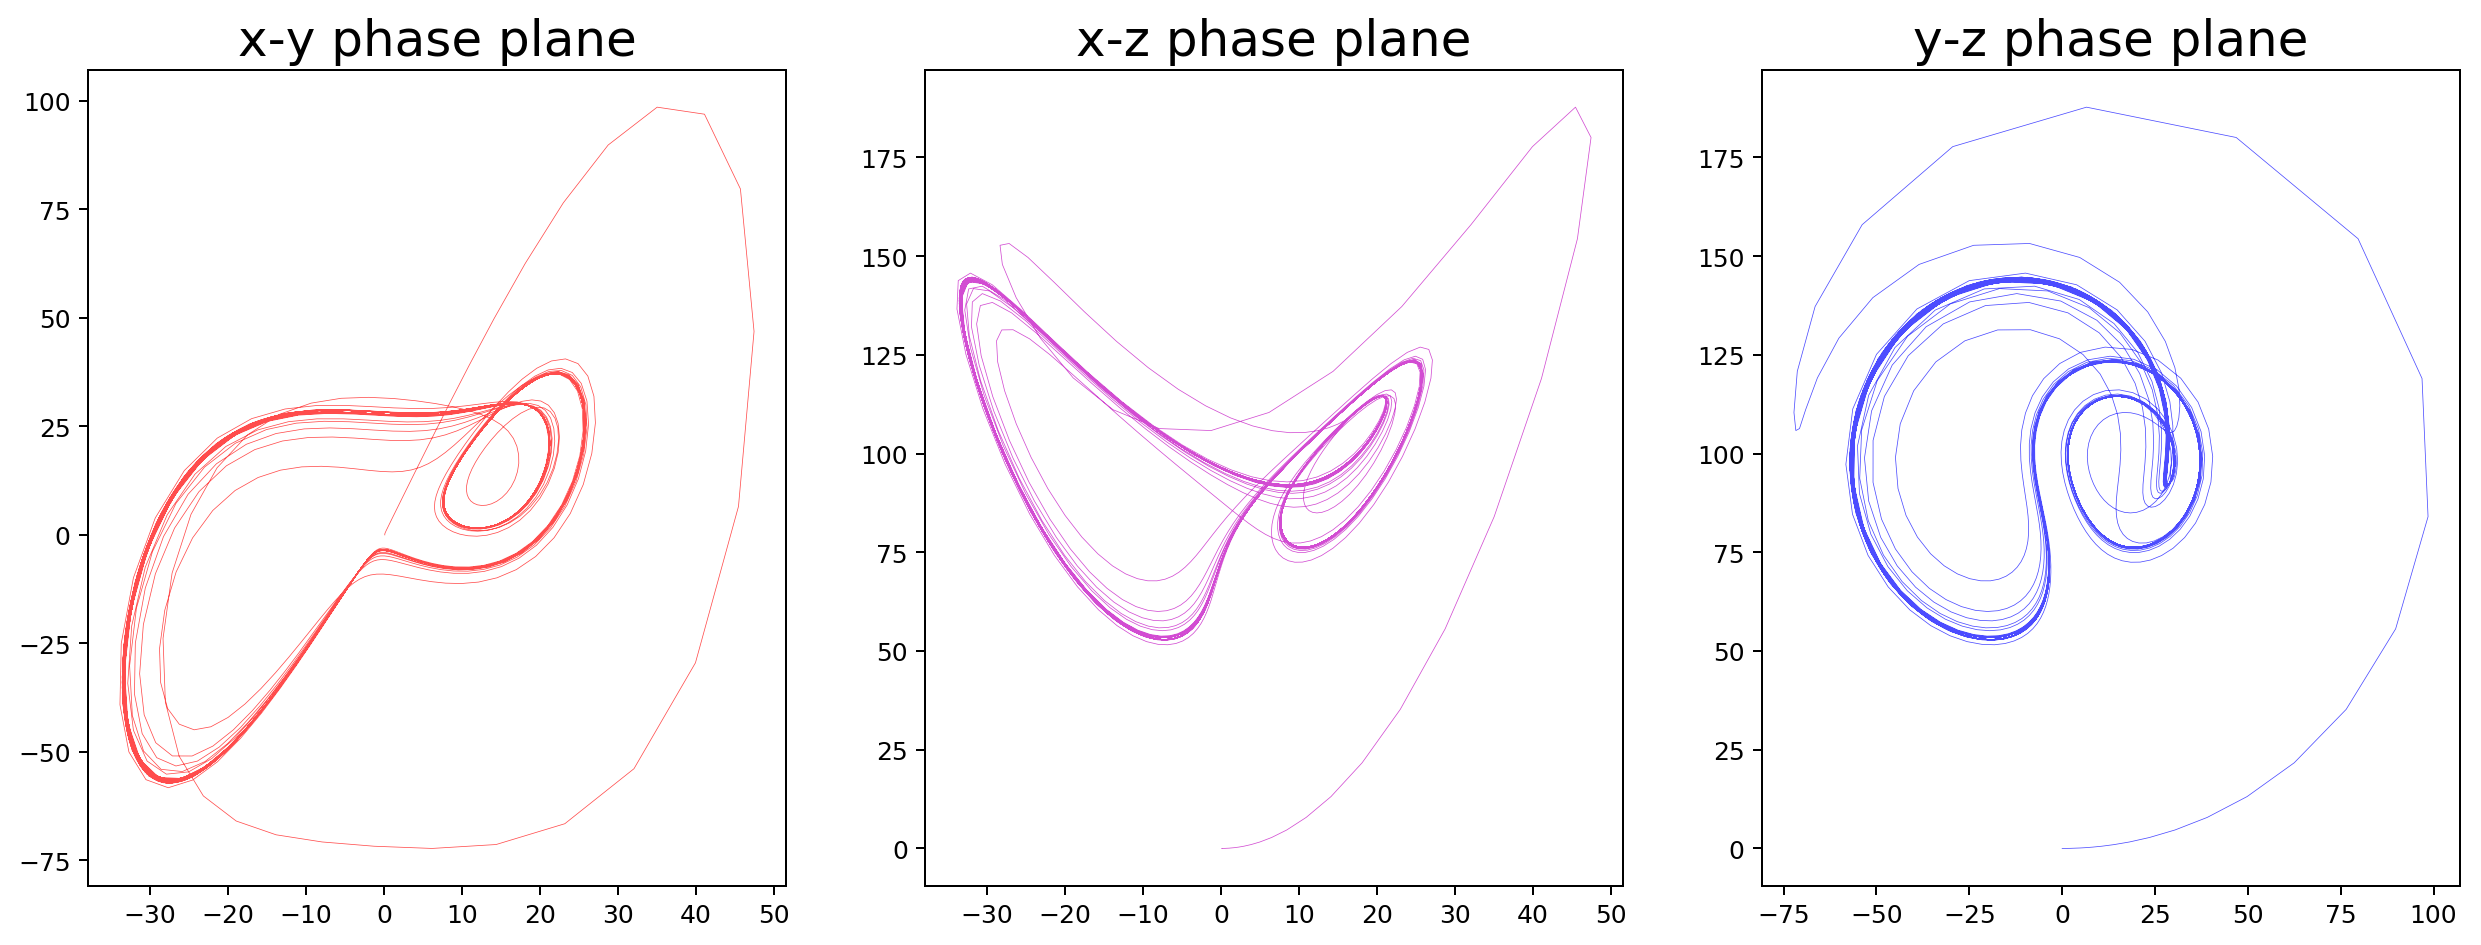
\includegraphics[width=0.6\linewidth]{lorenz-attractor-phase-plane3.png}
   \caption{Gráfica de Fase del Atractor de Lorenz en los planos.}
\end{figure}

La imagen nos presentan las fases en los planos XY, XZ y YZ respectivamente, que en este caso, como ya lo dijimos con la gráfica en el espacio, deja de mostrar grandes similitudes con las dos anteriores, pero aún así, mostrando formas interesantes. 

Por último tenemos:

\begin{figure}[ht!]
  \centering
  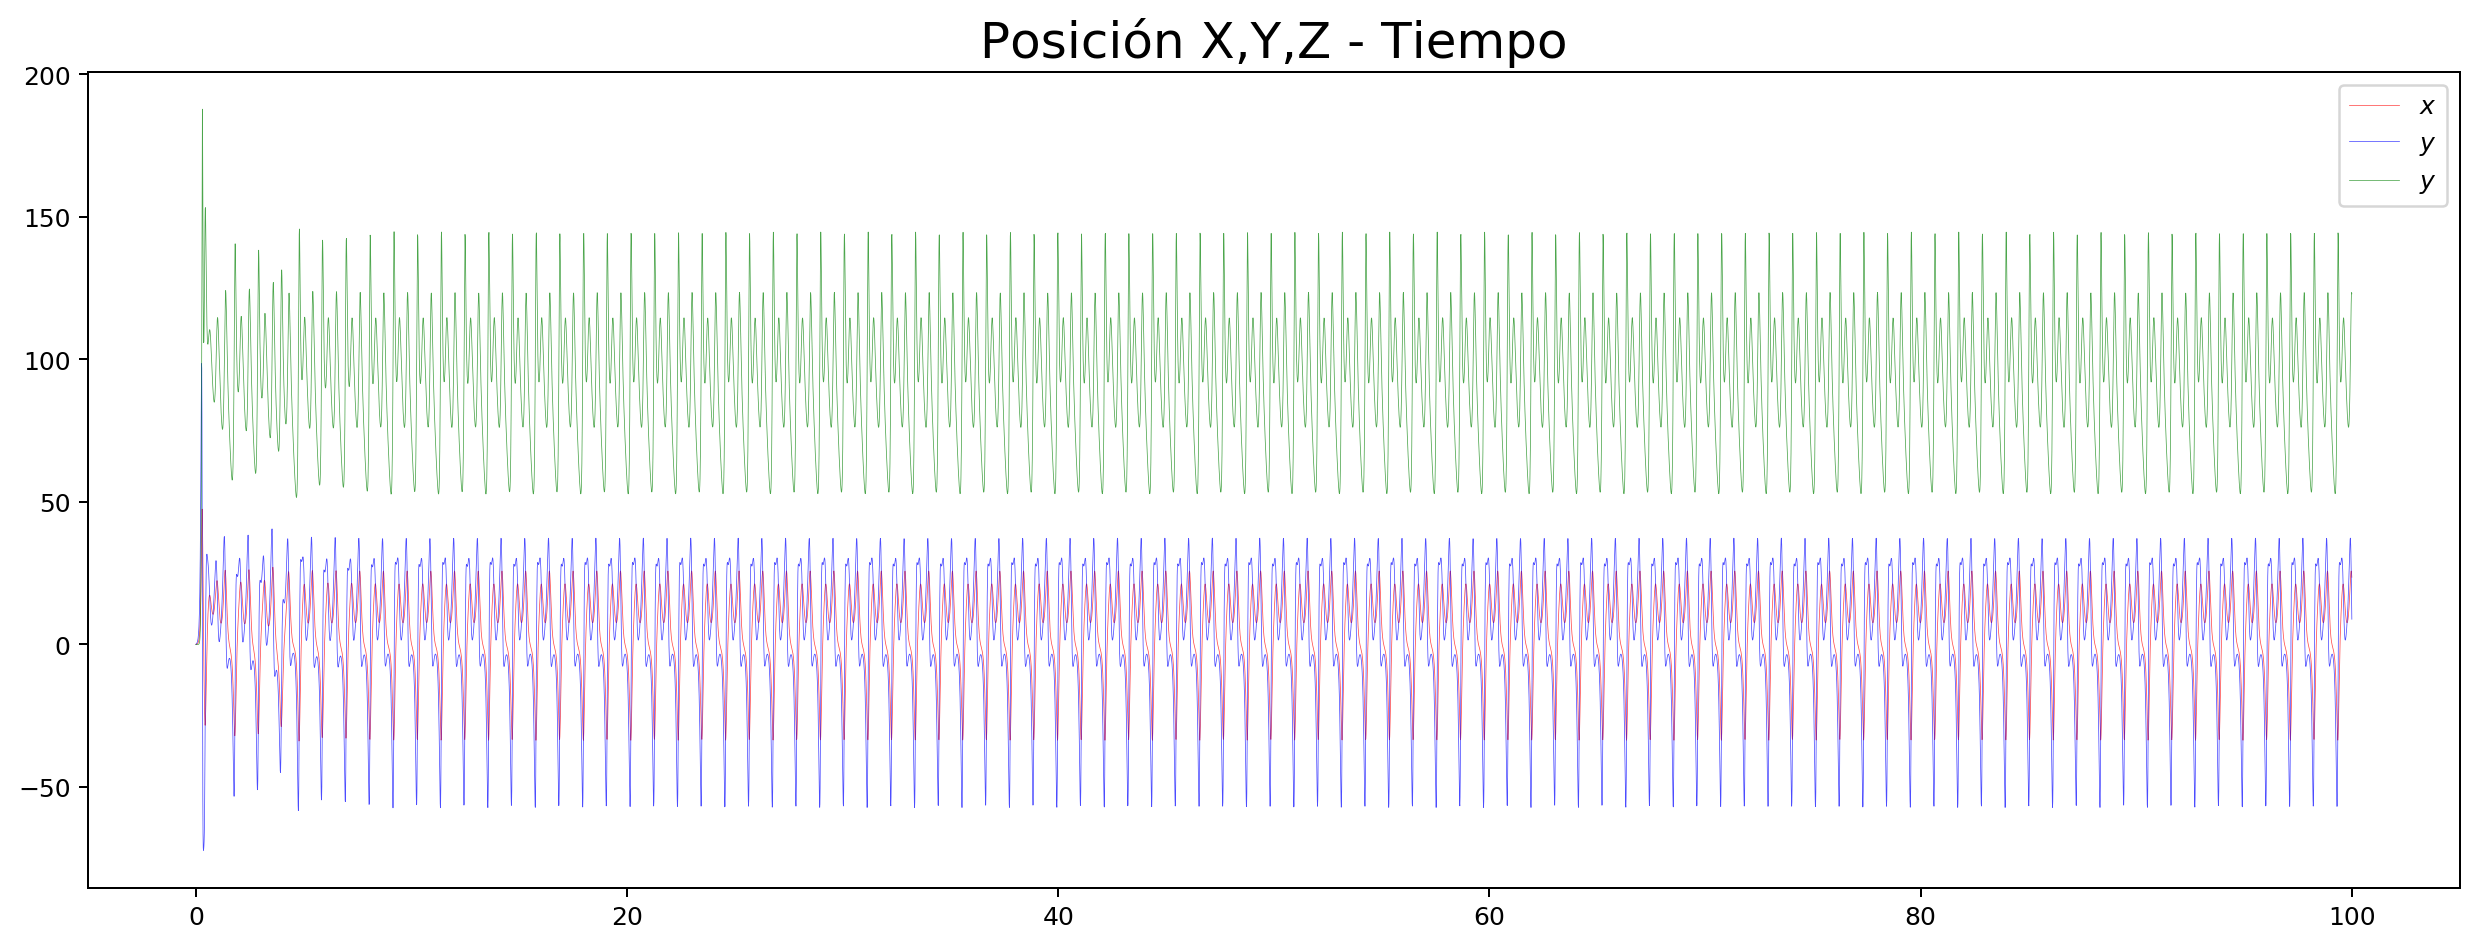
\includegraphics[width=0.6\linewidth]{lorenz-posicion-tiempo3.png}
   \caption{Posición con respecto al Tiempo}
\end{figure}

\begin{figure}[ht!]
  \centering
  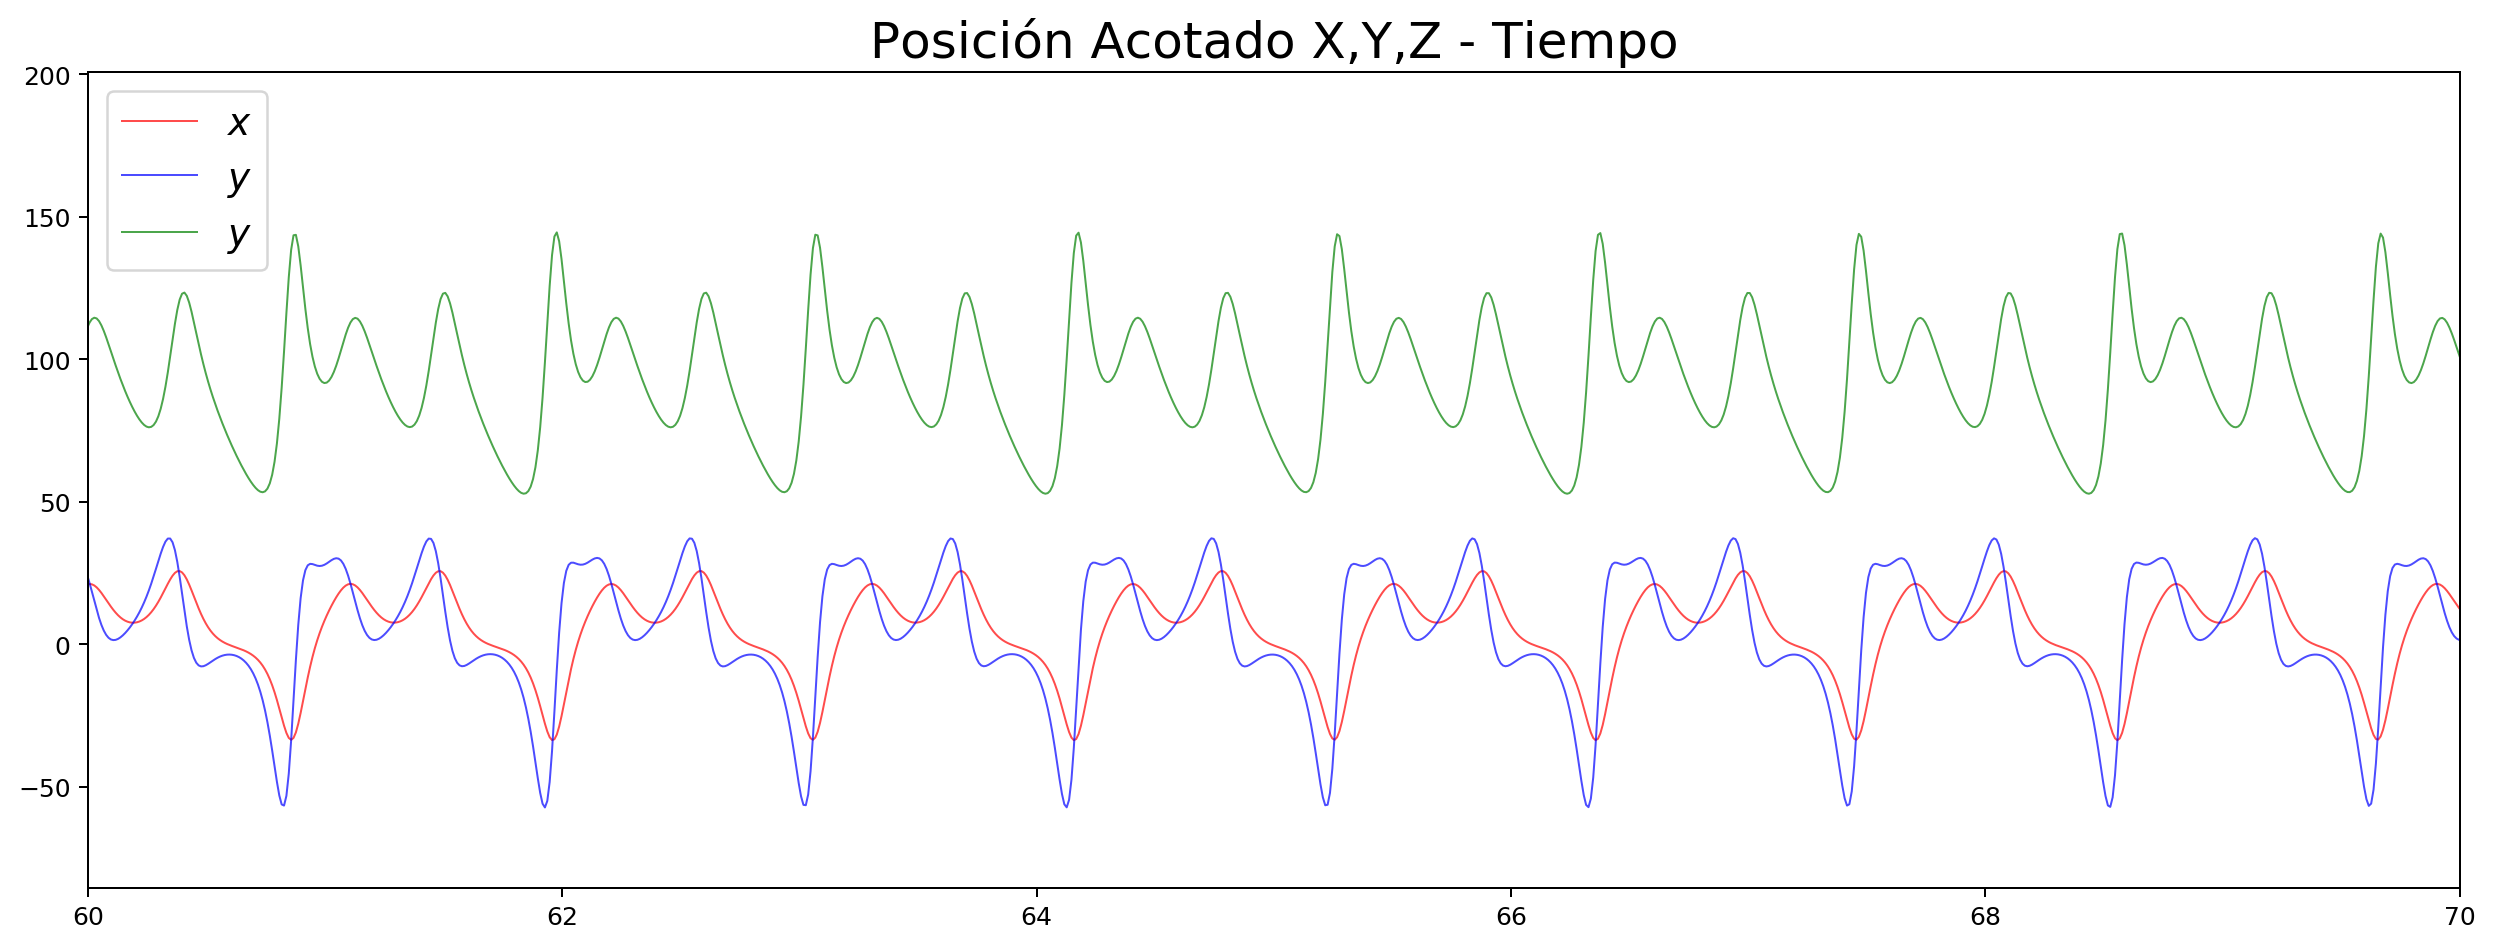
\includegraphics[width=0.6\linewidth]{lorenz-posicion-acotado-tiempo3.png}
  \caption{Posición con respecto al Tiempo}
\end{figure}

Aquí podemos observar las gráficas de posición de X, Y y Z con respecto al tiempo. En la segunda gráfica, donde mostramos más de cerca las posiciones. Ahora, podemos notar que X y Y ya no llevan un camino tan parecido, mientras que Z aún sigue estando posicionado más arriba. 

\section{Conclusión}
En cuanto al sistema de Lorenz, podemos concluir que las soluciones caóticas son muy evidentes al momento de mostrar las gráficas, ya que llevan formas muy parecidas, tal vez con pequeñas variaciones entre ellas.

En cuanto a la evaluación, se puede decir que ha sido muy interesante trabajar con lo aprendido de solución de ecuaciones diferenciales ordinarias. Gracias a las actividades hechas, hacer la evaluación no fue difícil, aunque las computadoras fallando al correr el código para la animación causó mucha frustración.

Por otra parte, cabe destacar que eso de hacer las animaciones fue muy interesante, es algo que no sabía que Python podía hacer, las gráficas  animadas resultaron muy llamativas.

\section{Bibliografía}
\begin{enumerate}
\item Boeing, G. (2016) Animating the Lorenz Attractor with Python. Recuperado el 26 de Abril del 2018 desde http://geoffboeing.com/2016/12/animating-lorenz-attractor-python/

\item Wikipedia (2018) Lorenz System. Recuperado el 26 de Abril del 2018 desde 

https://en.wikipedia.org/wiki/Lorenz\_system
\end{enumerate}

\end{document}